\begin{frame}{Resampling Data (No improvement)}
    \centering
    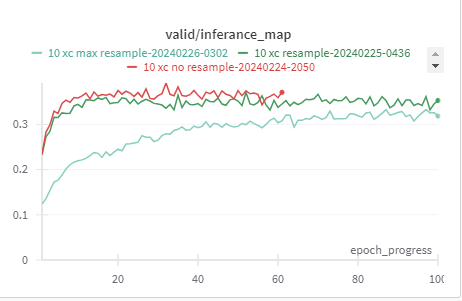
\includegraphics[height=0.7\textheight,width=0.7\textwidth,keepaspectratio]{images/resample.png}
\end{frame}

\begin{frame}{Mixitup (No improvement)}
    \centering
    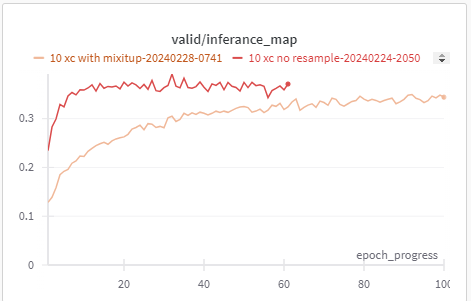
\includegraphics[height=0.7\textheight,width=0.7\textwidth,keepaspectratio]{images/mixitup.png}
\end{frame}

\begin{frame}{Notes on Data Augmentation}
    \centering
    \begin{itemize}
        \item Reverb is slow, todo
        \item Small changes in recent test
    \end{itemize}
\end{frame}

\begin{frame}{Far-Feild}
    \centering
    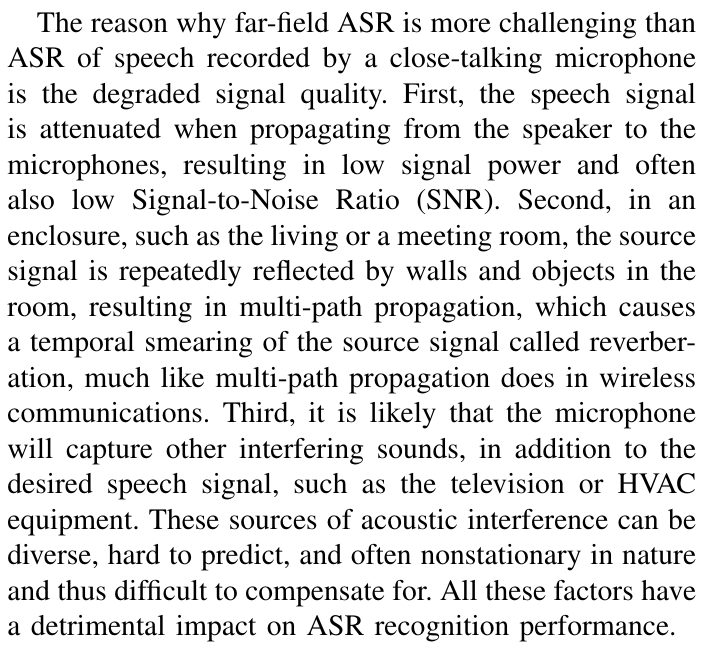
\includegraphics[height=0.7\textheight,width=0.7\textwidth,keepaspectratio]{images/FARFIELD.png}
    \begin{itemize}
        \item Far-Field Automatic Speech Recognition, Haeb-Umbach et. al, Lostanlen et. al
        \item Good models improve error by 20\% more channels by another 20\%
    \end{itemize}

\end{frame}

\begin{frame}{Far-Feild (Bioacoustics)}
    \centering
    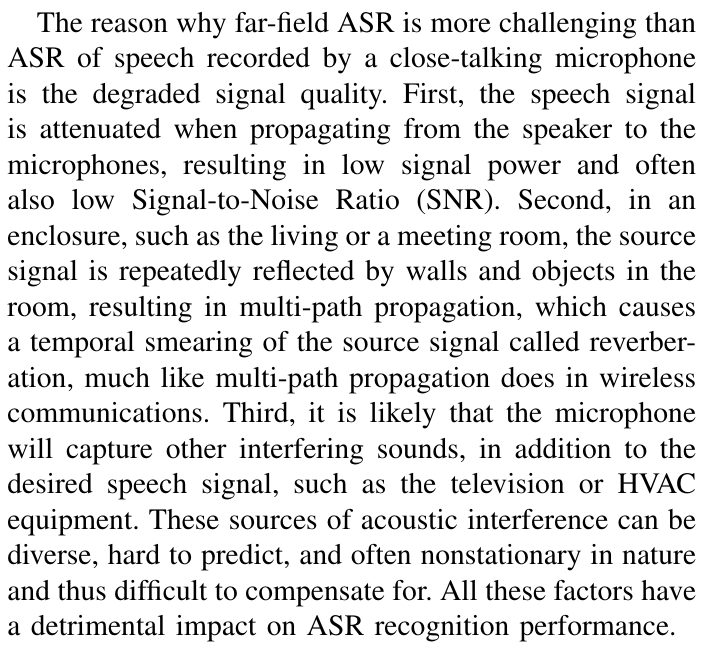
\includegraphics[height=0.7\textheight,width=0.7\textwidth,keepaspectratio]{images/FARFIELD.png}
    \begin{itemize}
        \item "Robust sound event detection in bioacoustic sensor networks", Lostanlen et. al
        \item AUC improvement from 61\% to 76\%
    \end{itemize}
\end{frame}

\begin{frame}{Next Steps}
    \centering
    \begin{itemize}
        \item Review augmentations
        \item ASR Lit Review
        \item Cloud Services
    \end{itemize}
\end{frame}

\begin{frame}{WTS Update}
    \centering
    \includegraphics[height=0.7\textheight,width=0.7\textwidth,keepaspectratio]{images/picture.png}
\end{frame}

%TODO DYLAN UPDATE HERE

% Slides for 2024-03-06
% To create a slide, use the following:
% \begin{frame}{TITLE}
%     BODY
% \end{frame}

% To create a slide with a bullet list, use the following:
% \begin{frame}{TITLE}
%     \begin{itemize}
%         \item ITEM 1
%         \item ITEM 2
%     \end{itemize}    
% \end{frame}

% To create a slide with numbered list, use the following:
% \begin{frame}{TITLE}
%     \begin{enumerate}
%         \item ITEM 1
%         \item ITEM 2
%     \end{enumerate}
% \end{frame}

% To create a slide with a graphic:
% 1. Add the graphic to this folder (named picture.png)
% 2. Use the following:
% \begin{frame}{TITLE}
%     \centering
%     \includegraphics[height=0.7\textheight,width=0.7\textwidth,keepaspectratio]{picture.png}
% \end{frame}

% To create a slide with two columns, use the following:
% \begin{frame}{TITLE}
%     \begin{columns}
%         \begin{column}{0.5\textwidth}
%             COLUMN 1 BODY
%         \end{column}
%         \begin{column}{0.5\textwidth}
%             COLUMN 2 BODY
%         \end{column}
%     \end{columns}
% \end{frame}
